\titleformat {\chapter} {\normalfont\huge\bfseries\color{black}}   {\thechapter}{10pt}{\huge} 
\chapter {Simulation Results}

%% ================================
%% \input{Advice-on-Chapter-4}
%% ================================
	
\section{The Parametric Equations}
%% \label{sec:4.1-CNC-Research-Machine}

The ten(10) 2D parametric curves covered in this work are:
\begin{enumerate}
	\item Teardrop
	\item Butterfly
	\item Ellipse
	\item Skewed-Astroid
	\item Circle
	\item AstEpi = Astroid + Epicycloid combination
	\item Snailshell
	\item SnaHyp = Snailshell + Hypotrocoid combination
	\item Ribbon-10L
	\item Ribbon-100l = 10 times scaleup of Ribbon-10L
	
\end{enumerate}

The parametric equations describing each of the curves x(u), and y(u) are provided in the next table. The independent parameter u is limited to
\begin{equation}
u  \in  [0.0, 1.0] \nonumber
\end{equation}

The curves were selected based on their different characteristics like closed loop curves, open ended curves, symmetric or non-symmetric about the x-axis and y-axis, and having concave or convex turns. The x and y dimensions (sizes) vary among the different curves. \vspace*{1\baselineskip}

The main objective of the selection criteria is to ensure that the interpolation algorithm for the parametric curve succeeds and does not break in all cases. \vspace*{1\baselineskip}
	
The results for the feedrates in machining the ten(10) curves show continuity, smoothness, with no abrupt jumps as the CNC machine traverse the entire curve from the start (u = 0.0) until the end (u = 1.0).	\vspace*{1\baselineskip}
		
\pagebreak
%% ================================================
%% \subsection{Teardrop and Butterfly equations}
\begin{table}[ht]
	\begin{center}
		\begin{tabular}[top]{ |p{16.0 cm}| }
			\rowcolor{LIGHTCYAN}			
			%% \hline \multicolumn{1}{|c|}{\textbf{Part 1/5 Teardrop and Butterfly parametric curves}} \\ [1.0ex]
	
			\hline \textbf{No. 1 - Teardrop parametric curve} \\
			 \begin{eqnarray}
			 x(u) & = & - 150u + 450u^2 - 300u^3 \nonumber \\   
			 y(u) & = & - 150u + 150u^2 \nonumber \\
			 u & \in & [0.0, 1.0] \nonumber
			\end{eqnarray}
		
			 Closed loop\\
			 Overall Single loop\\
			 Reflection x-axis: non-symmetrical\\
			 Reflection y-axis: symmetrical\\
			 \frame{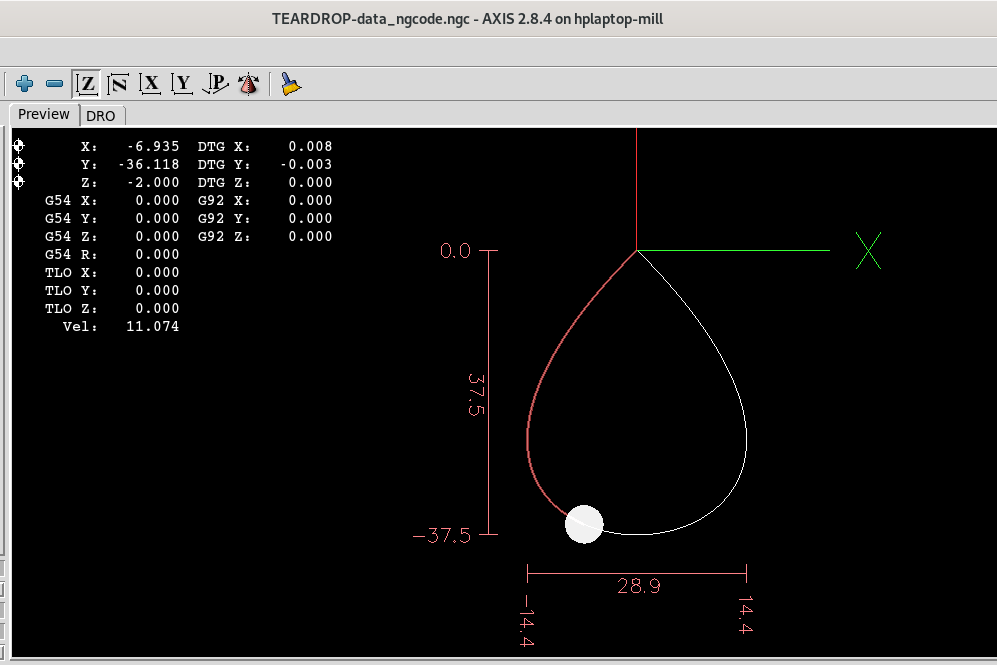
\includegraphics[width=0.565\textwidth]{./07-images/img-Ch5/TEARDROP-Axis.png}}
			 \frame{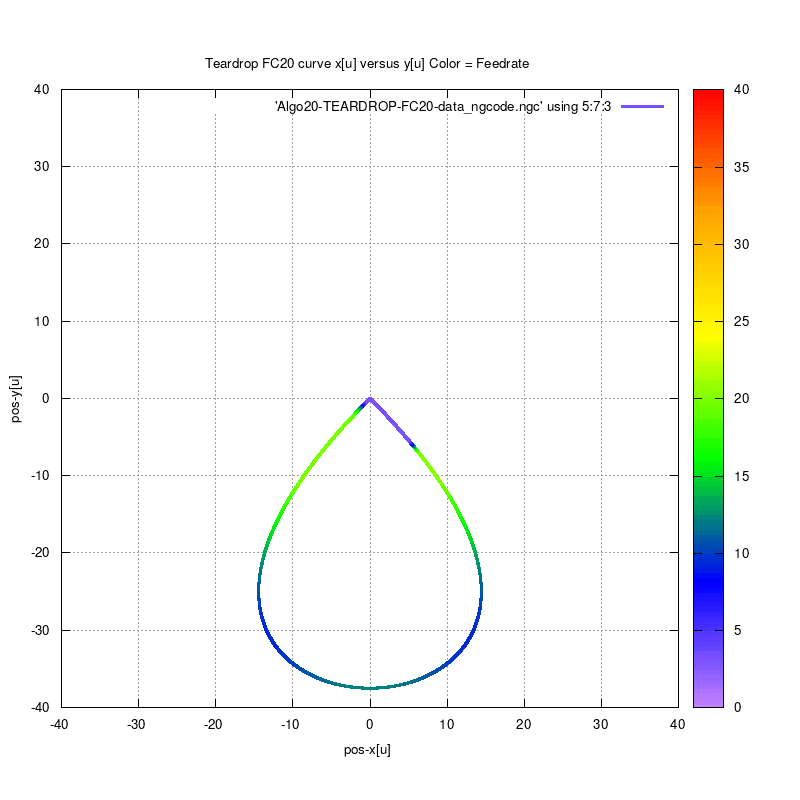
\includegraphics[width=0.38\textwidth]{./07-images/img-Ch5/TEARDROP-Feedrate.png}}\\
			
			\rowcolor{LIGHTCYAN}
			\hline \textbf{No. 2 - Butterfly parametric curve}\\
			\begin{eqnarray}
				x(u) & = & \sin(2\pi u) \left [ e^{\cos(2\pi u)} - 2\cos(8\pi u) - (\sin(2\pi u/12))^5 \right] \nonumber \\
				y(u) & = & \cos(2\pi u) \left [ e^{\cos(2\pi u)} - 2\cos(8\pi u) - (\sin(2\pi u/12))^5 \right] \nonumber \\
				u & \in & [0.0, 1.0] \nonumber
			\end{eqnarray}
			      
			
			Closed loop\\
			Overall Multiple loops\\
			Reflection x-axis: non-symmetrical\\
			Reflection y-axis: symmetrical\\
			\frame{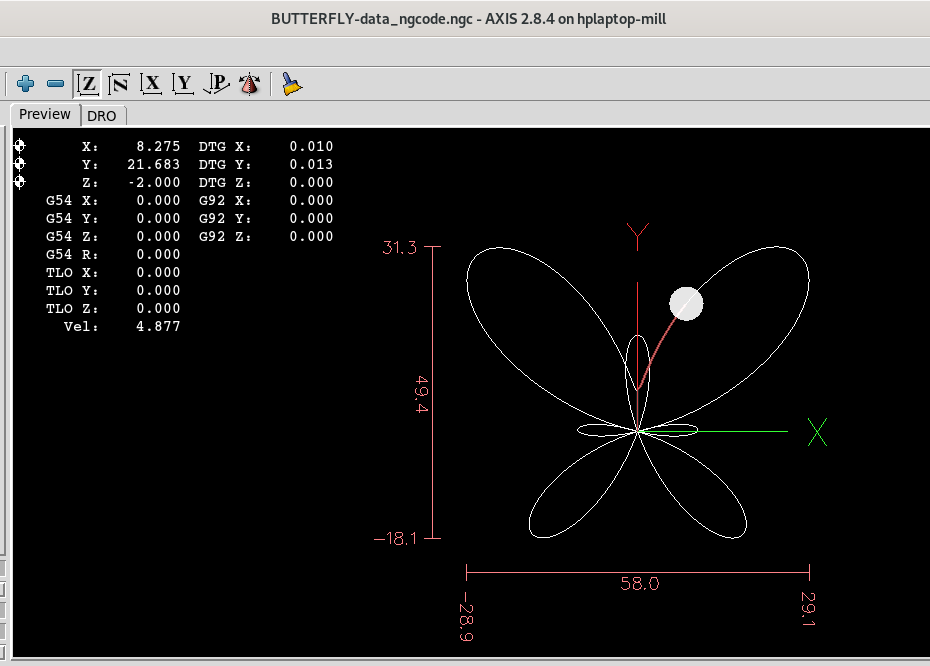
\includegraphics[width=0.56\textwidth]{./07-images/img-Ch5/BUTTERFLY-Axis.png}}
            \frame{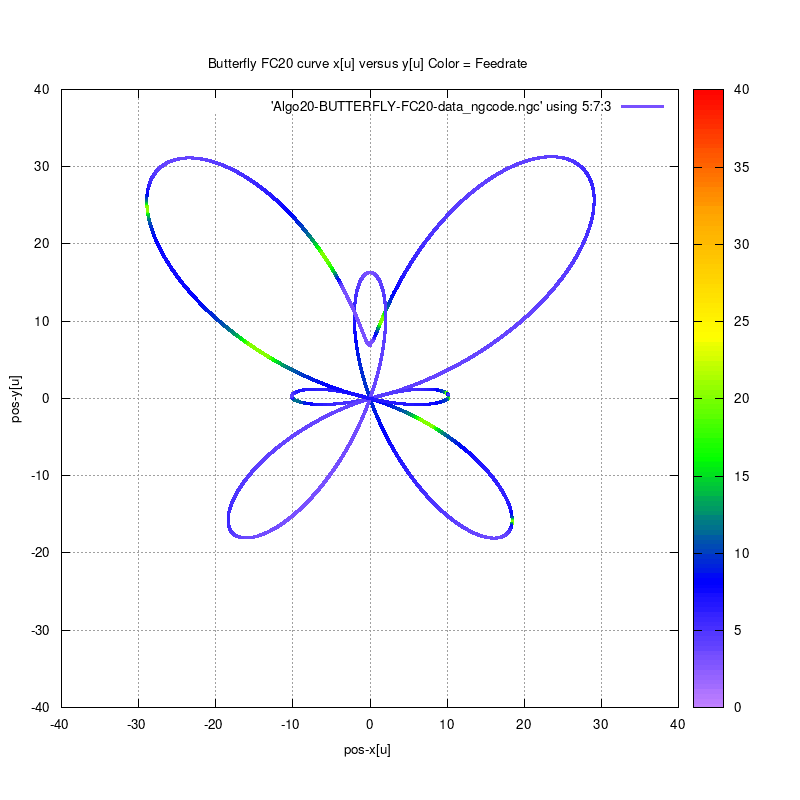
\includegraphics[width=0.40\textwidth]{./07-images/img-Ch5/BUTTERFLY-Feedrate.png}}\\

			\hline
		\end{tabular}
		%% \caption{Equations and dimensions of Teardrop and Butterfly curves}		
		\label{table:Part1of5 Equations and dimensions of the parametric curves}
	\end{center}
\end{table}  

\pagebreak

%% ================================================
%% \subsection{Ellipse and Skewed-Astroid equations}

\begin{table}[ht]
	\begin{center}
		\begin{tabular}[top]{ |p{16.0 cm}| }
			\rowcolor{LIGHTCYAN}			
		%%	\hline \multicolumn{1}{|c|}{\textbf{Part 2/5 Ellipse and Skewed-Astroid parametric curves}} \\ [1.0ex]
			
			
		%%	 // ELLIPSE X
		%%	double scaleup = 11.0;
		%%	double k = (2.0 * PI_cpos);
		%%	double x = sin(k*u);
		%%	return (scaleup)*(x);
			
			
			\hline \textbf{No. 3 - Ellipse parametric curve} \\
			\begin{eqnarray}
				x(u) & = & 11\sin(2\pi u) \nonumber \\   
				y(u) & = & 51\cos(2\pi u) \nonumber \\
				u & \in & [0.0, 1.0] \nonumber
			\end{eqnarray}
			
			Closed loop\\
			Overall Single loop, smooth convex curves\\
			Reflection x-axis: symmetrical\\
			Reflection y-axis: symmetrical\\
			\frame{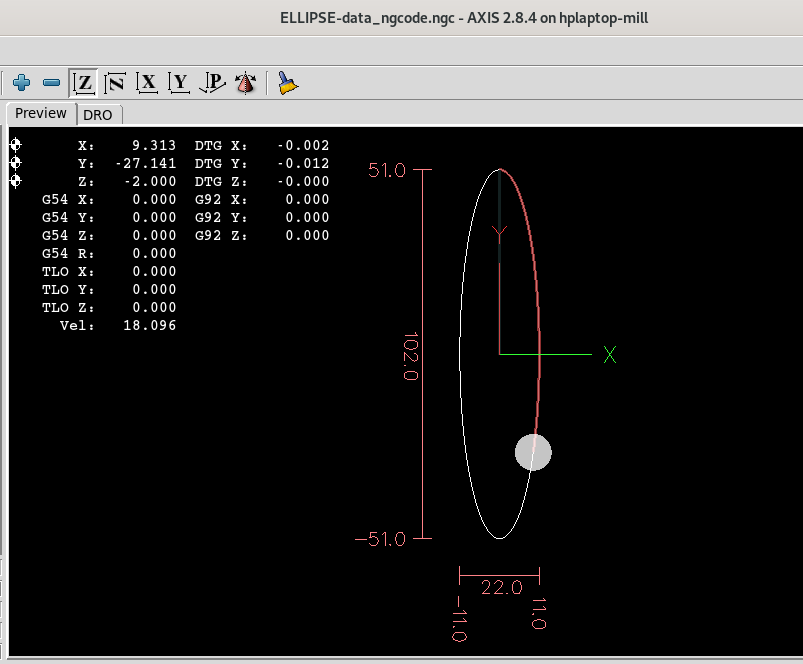
\includegraphics[width=0.51\textwidth]{./07-images/img-Ch5/ELLIPSE-Axis.png}}
			\frame{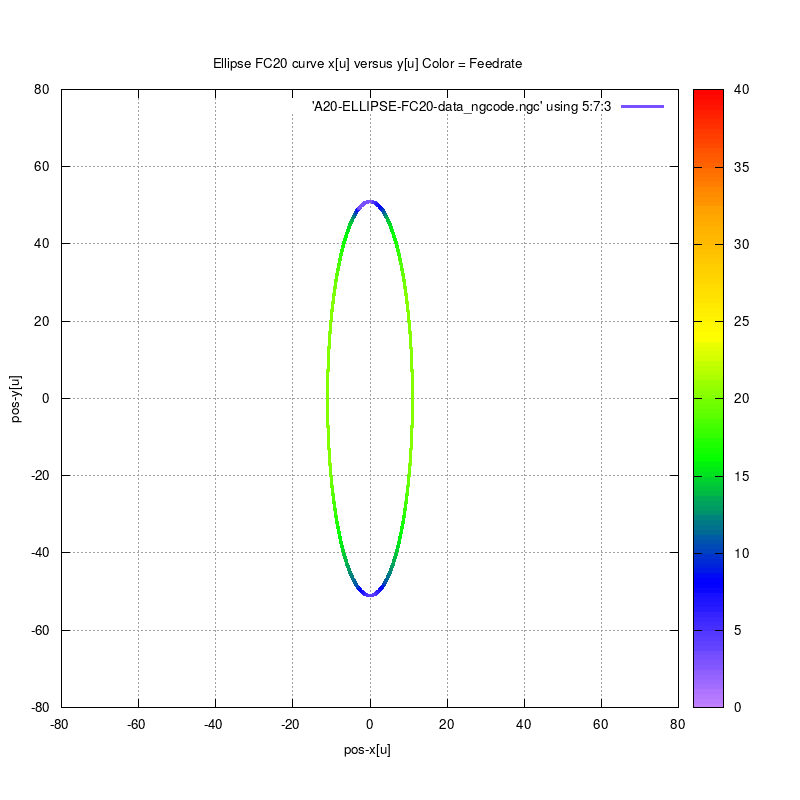
\includegraphics[width=0.42\textwidth]{./07-images/img-Ch5/ELLIPSE-Feedrate.png}}\\
			
			\rowcolor{LIGHTCYAN}
			\hline \textbf{No. 4 - Skewed-Astroid parametric curve}\\
			\begin{eqnarray}
				x(u) & = & 40  [ \sin(2\pi u) ]^3  \nonumber \\
				y(u) & = & 100 [ \cos(2\pi u) ]^3  \nonumber \\
				u & \in & [0.0, 1.0] \nonumber
			\end{eqnarray}
			
			
			Closed loop\\
			Overall Single loop, 4 cusps and 4 concave curves \\
			Reflection x-axis: symmetrical\\
			Reflection y-axis: symmetrical\\
			\frame{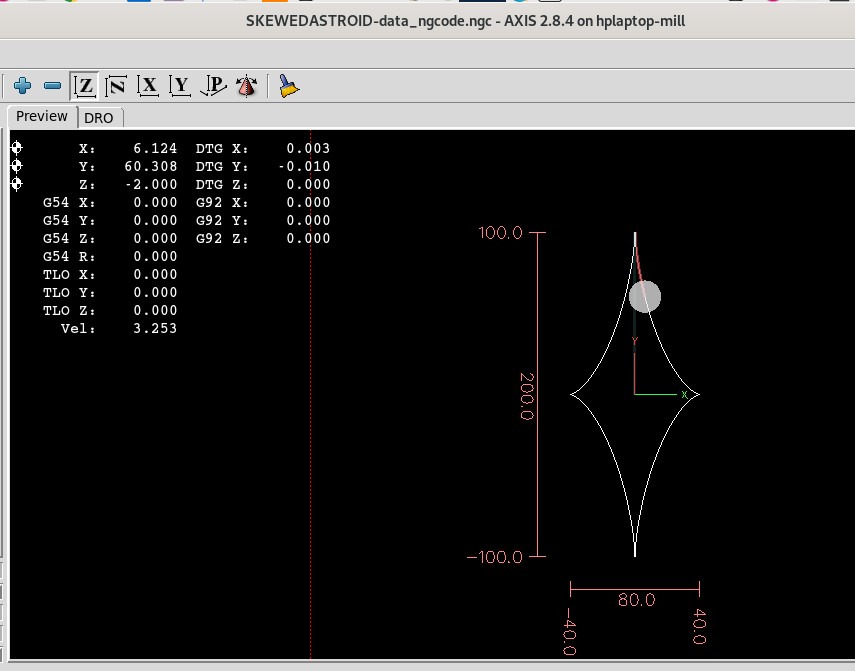
\includegraphics[width=0.51\textwidth]{./07-images/img-Ch5/SKEWED-ASTROID-Axis.png}}
			\frame{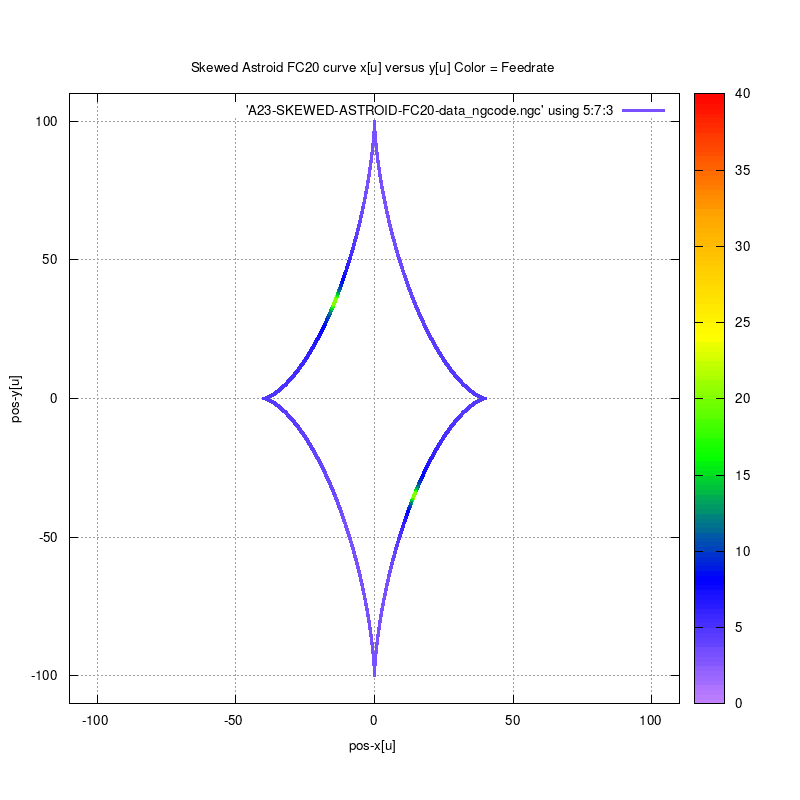
\includegraphics[width=0.40\textwidth]{./07-images/img-Ch5/SKEWED-ASTROID-Feedrate.png}}\\
			
			\hline
		\end{tabular}
		%% \caption{Equations and dimensions of Teardrop and Butterfly curves}		
		\label{table:Part2of5 Equations and dimensions of the parametric curves}
	\end{center}
\end{table}  

\pagebreak

%% ================================================
%% \subsection{Circle and AstEpi equations}

\begin{table}[ht]
	\begin{center}
		\begin{tabular}[top]{ |p{16.0 cm}| }
			\rowcolor{LIGHTCYAN}			
		%%	\hline \multicolumn{1}{|c|}{\textbf{Part 3/5 Circle and AstEpi parametric curves}} \\ [1.0ex]

			\hline \textbf{No. 5 - Circle parametric curve} \\
			\begin{eqnarray}
				x(u) & = & 79\sin(2\pi u) \nonumber \\   
				y(u) & = & 79\cos(2\pi u) \nonumber \\
				u & \in & [0.0, 1.0] \nonumber
			\end{eqnarray}
			
			Closed loop\\
			Overall Single loop, smooth convex curves\\
			Reflection x-axis: symmetrical\\
			Reflection y-axis: symmetrical\\
			\frame{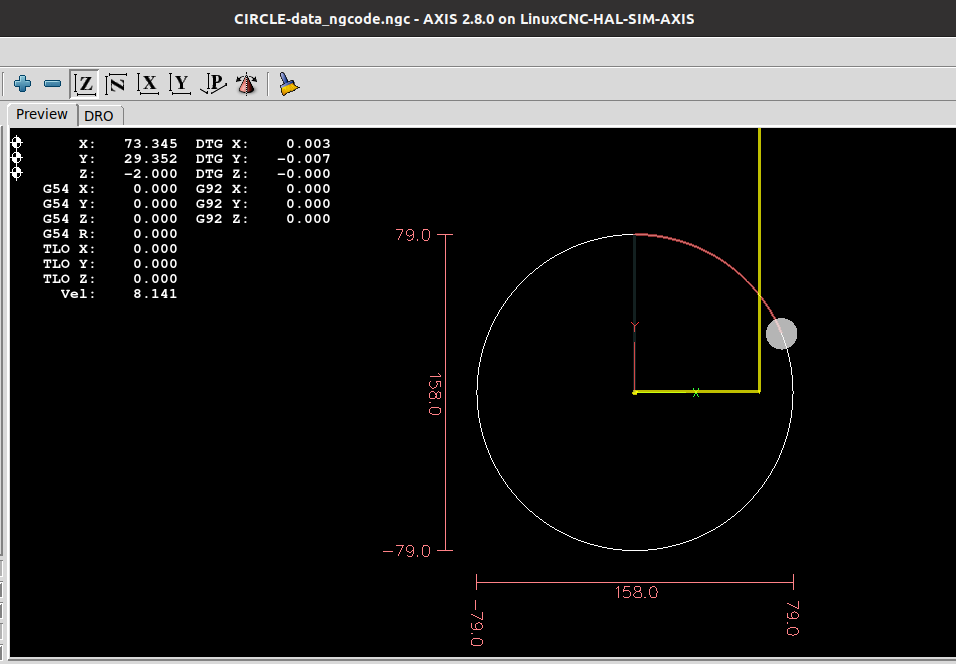
\includegraphics[width=0.560\textwidth]{./07-images/img-Ch5/CIRCLE-Axis.png}}
			\frame{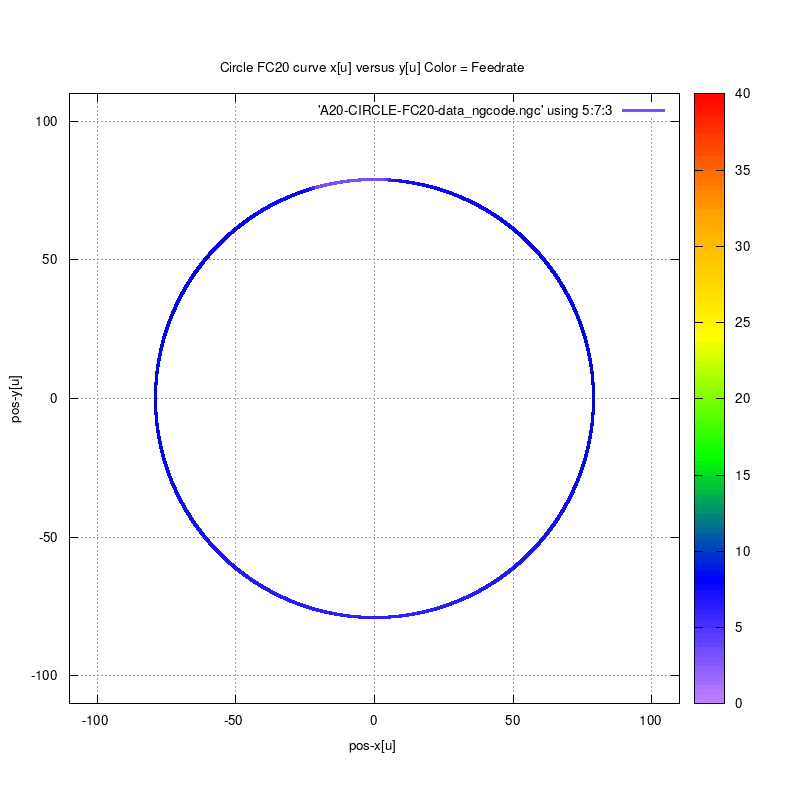
\includegraphics[width=0.394\textwidth]{./07-images/img-Ch5/CIRCLE-Feedrate.png}}\\
			
            \rowcolor{LIGHTCYAN}
			\hline \textbf{No. 6 - AstEpi = Sum of (Astroid + Epicycloid) parametric curves}\\
			
			\begin{eqnarray}
				tiny & = & 1.0\tenpow{-10} \nonumber \\
				x(u) & = & 40[\sin(2\pi u)]^3 + 50\cos(2\pi u + tiny) - 10\cos(10\pi u -tiny) \nonumber \\
				y(u) & = & 40[\cos(2\pi u)]^3 + 50\sin(2\pi u + tiny) - 10\sin(10\pi u -tiny) \nonumber \\
				u & \in & [0.0, 1.0] \nonumber
			\end{eqnarray}
			
			
			Closed loop\\
			Overall Three loops, all convex curves \\
			Reflection x-axis: non-symmetrical\\
			Reflection y-axis: non-symmetrical\\
			\frame{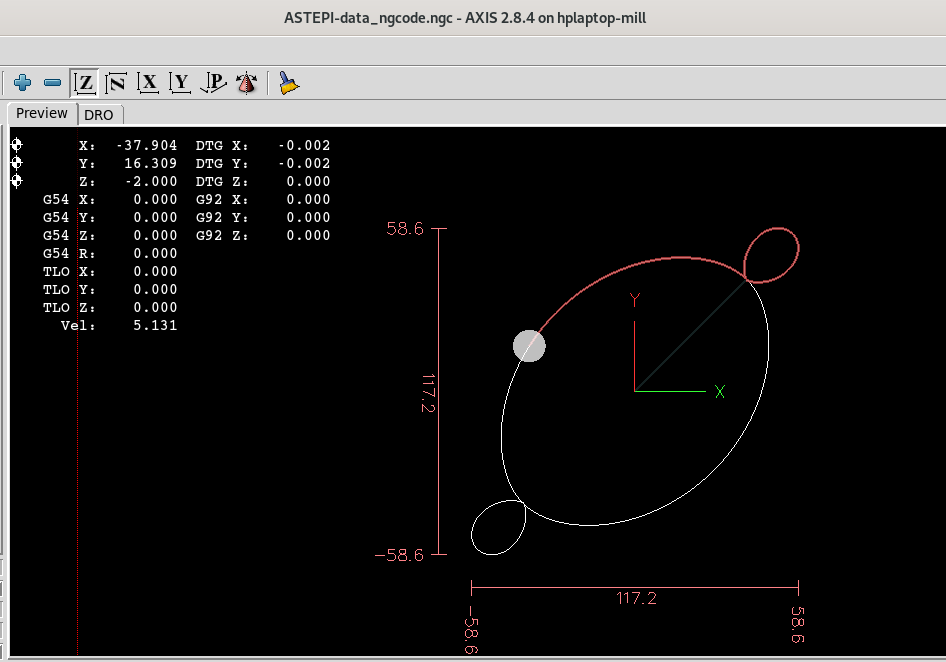
\includegraphics[width=0.560\textwidth]{./07-images/img-Ch5/ASTEPI-Axis.png}}
			\frame{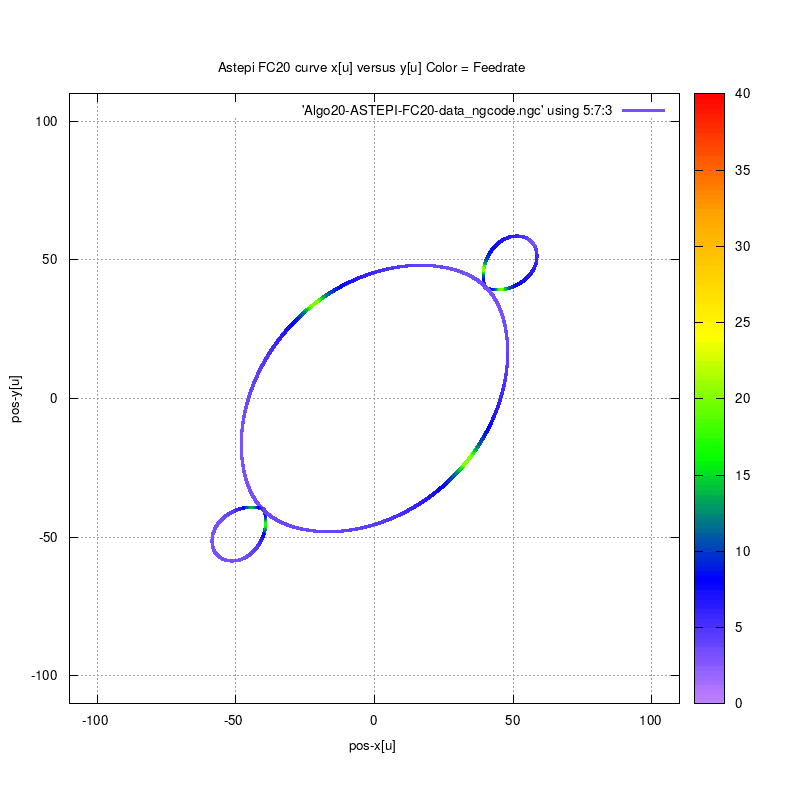
\includegraphics[width=0.395\textwidth]{./07-images/img-Ch5/ASTEPI-Feedrate.png}}\\
			
			\hline
		\end{tabular}
		%% \caption{Equations and dimensions of Teardrop and Butterfly curves}		
		\label{table:Part3of5 Equations and dimensions of the parametric curves}
	\end{center}
\end{table}  

\pagebreak

%% ================================================
%% \subsection{Snailshell and SnaHyp equations}

\begin{table}[ht]
	\begin{center}
		\begin{tabular}[top]{ |p{16.0 cm}| }
			\rowcolor{LIGHTCYAN}			
			%% \hline \multicolumn{1}{|c|}{\textbf{Part 4/5 Snailshell and SnaHyp parametric curves}} \\ [1.0ex]
 

%% double scaleup = 100.0;
%% double k = (3.0*PI_cpos);
%% double x = ( sin(2*k*u) / (k*u*k*u + 4.0) );
%% return (scaleup)*(x);

%% double scaleup = 100.0;
%% double k = (3.0*PI_cpos);
%% double y = (cos(2*k*u) / (k*u*k*u + 4.0));
%% return (scaleup)*(y);
			
			\hline \textbf{No. 7 - Snailshell parametric curve}\\
			\begin{eqnarray}
				x(u) & = & 100\sin(6\pi u) / [9 (\pi u)^2 + 4] \nonumber \\   
				y(u) & = & 100\cos(6\pi u) / [9 (\pi u)^2 + 4] \nonumber \\
				u & \in & [0.0, 1.0] \nonumber
			\end{eqnarray}
			
			Open ended curve\\
			Overall No loop, smooth and continuous convex curves\\
			Reflection x-axis: non-symmetrical\\
			Reflection y-axis: non-symmetrical\\
			\frame{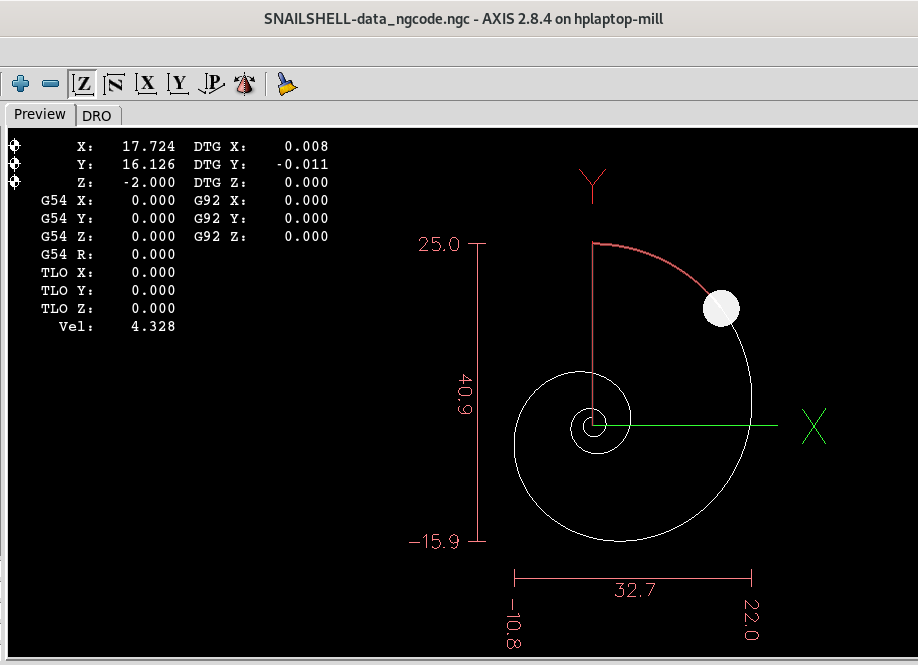
\includegraphics[width=0.550\textwidth]{./07-images/img-Ch5/SNAILSHELL-Axis.png}}
			\frame{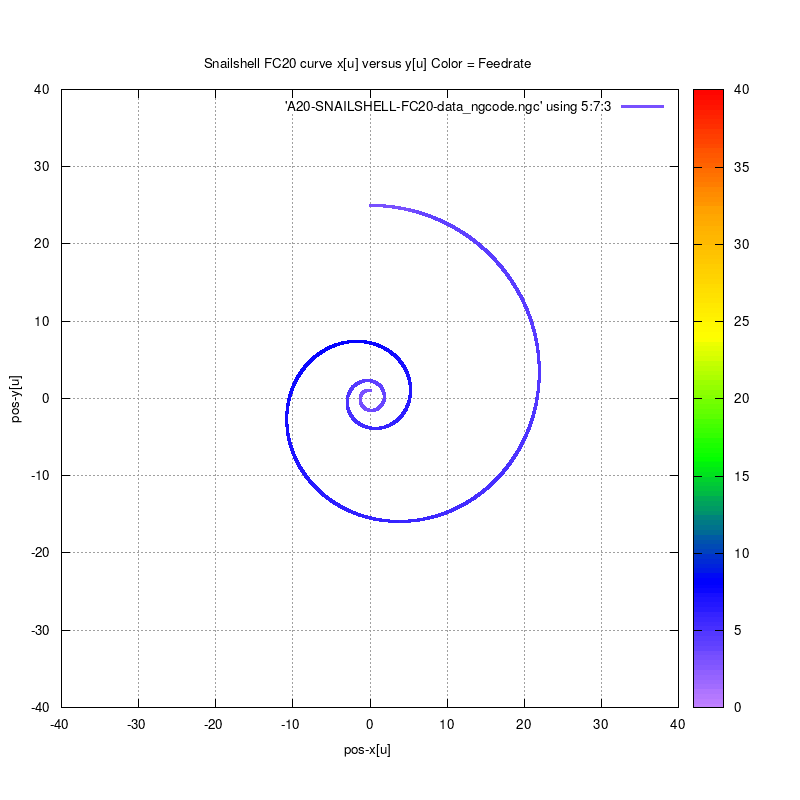
\includegraphics[width=0.395\textwidth]{./07-images/img-Ch5/SNAILSHELL-Feedrate.png}}\\
			 
			\rowcolor{LIGHTCYAN}
			\hline \textbf{No. 8 - SnaHyp = Sum of (Snailshell + Hypotrocoid) parametric curves}\\

			\begin{eqnarray}
				xsna(u) & = & [4\sin(8\pi u) ] / [16 (\pi u)^2 + 4] \nonumber \\
				xhyp(u) & = & [2\cos(4\pi u)  + 5\cos(8\pi u /3)  ] \nonumber \\
				x(u) & = & 10[xsna(u) + xhyp(u)] \nonumber \\
			    ysna(u) & = & [10\cos(8\pi u)] / [16 (\pi u)^2 + 4] \nonumber \\
				yhyp(u) & = & [2\sin(8\pi u) - 5\sin(8\pi u /3)] \nonumber \\
				y(u) & = & 10[ysna(u) + yhyp(u)] \nonumber \\
				u & \in & [0.0, 1.0] \nonumber
			\end{eqnarray}

%% double scaleup = 10.0;
%% double k = (4.0 * PI_cpos);
%% double small = 1.0e-10;
%% double x_sna = (4.0)*( sin(2*k*u) / (k*u*k*u + 4.0) );
%% double x_hyp = (2*cos(k*u) + 5*cos(2*k*u/3));
%% double x = x_sna + x_hyp;
%% return (scaleup)*(x);

%% double scaleup = 10.0;
%% double k = (4.0 * PI_cpos);
%% double small = 1.0e-10;
%% double y_sna = (10)*(cos(2*k*u) / (k*u*k*u + 4.0));
%% double y_hyp = (2*sin(k*u) - 5*sin(2*k*u/3));
%% double y = y_sna + y_hyp;
%% return (scaleup)*(y);			
			
			Open ended curve\\
			Overall 1 loop, except for 1 concave curve, the rest are convex curves \\
			Reflection x-axis: non-symmetrical\\
			Reflection y-axis: non-symmetrical\\
			\frame{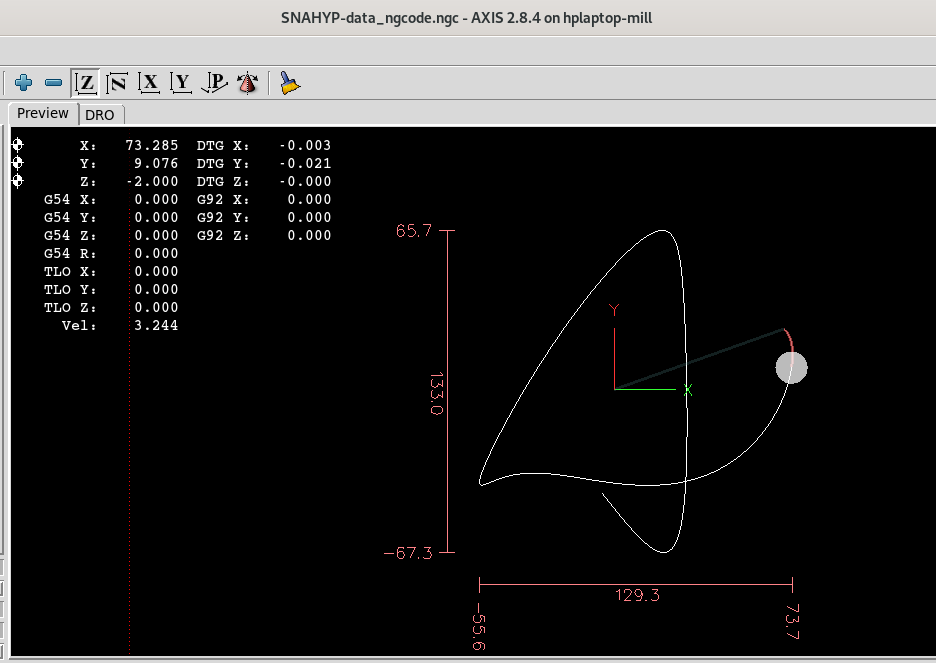
\includegraphics[width=0.560\textwidth]{./07-images/img-Ch5/SNAHYP-Axis.png}}
			\frame{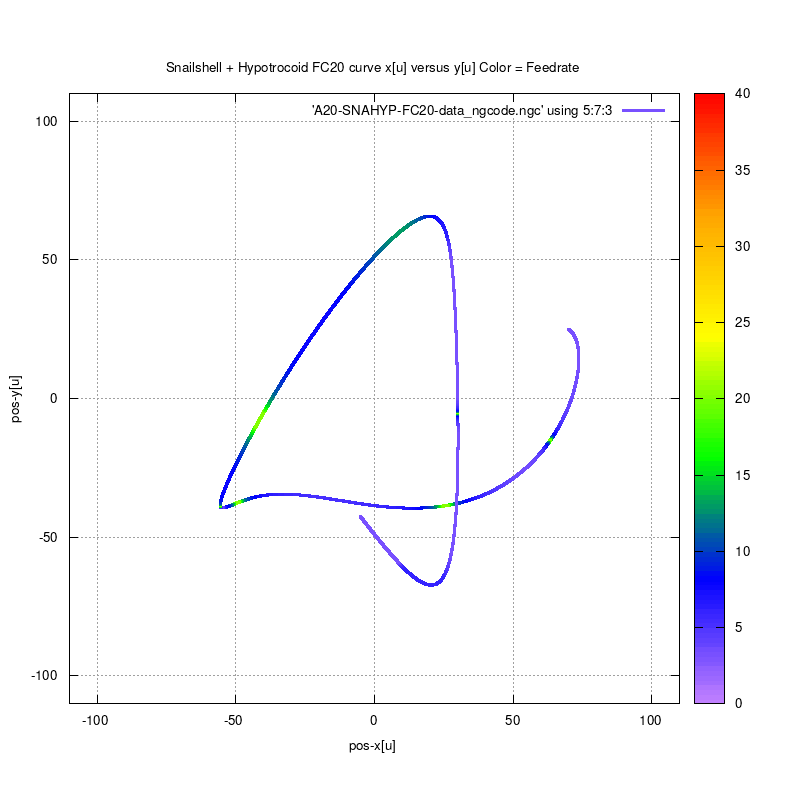
\includegraphics[width=0.395\textwidth]{./07-images/img-Ch5/SNAHYP-Feedrate.png}}\\
			
			\hline
		\end{tabular}
		%% \caption{Equations and dimensions of Teardrop and Butterfly curves}		
		\label{table:Part4of5 Equations and dimensions of the parametric curves}
	\end{center}
\end{table}  

\pagebreak

%% ================================================
%% \subsection{Ribbon-10L and Ribbon-100L equations}
\begin{table}[ht]
	\begin{center}
		\begin{tabular}[top]{ |p{16.0 cm}| }
			\rowcolor{LIGHTCYAN}			
			%% \hline \multicolumn{1}{|c|}{\textbf{Part 5/5 Circle and AstEpi parametric curves}} \\ [1.0ex]
			
	%%	double t = 4.0*(u - 0.50); // TRANSORMATION EQUATION
	%%	double scaleup = 1.0;
	%%	double x = (t*t);
	%%	return (scaleup)*(x);	
			
	%%	double t = 4.0*(u - 0.50); // TRANSORMATION EQUATION
	%% 	double scaleup = 1.0;
	%%	double y = (t*t*t) - 3*(t) + 3;
	%%	return (scaleup)*(y);
			
			
			\hline  \textbf{No. 9 - Ribbon-10L parametric curve}\\
			\begin{eqnarray}
				t(u) & = & 4(u - 0.50) \nonumber \\
				x(u) & = & t^2 \nonumber \\   
				y(u) & = & t^3 - 3t + 3 \nonumber \\
				u & \in & [0.0, 1.0] \nonumber
			\end{eqnarray}
			
			Open ended curve\\
			Overall Single loop, smooth convex curves\\
			Reflection x-axis: non-symmetrical\\
			Reflection y-axis: non-symmetrical\\
			\frame{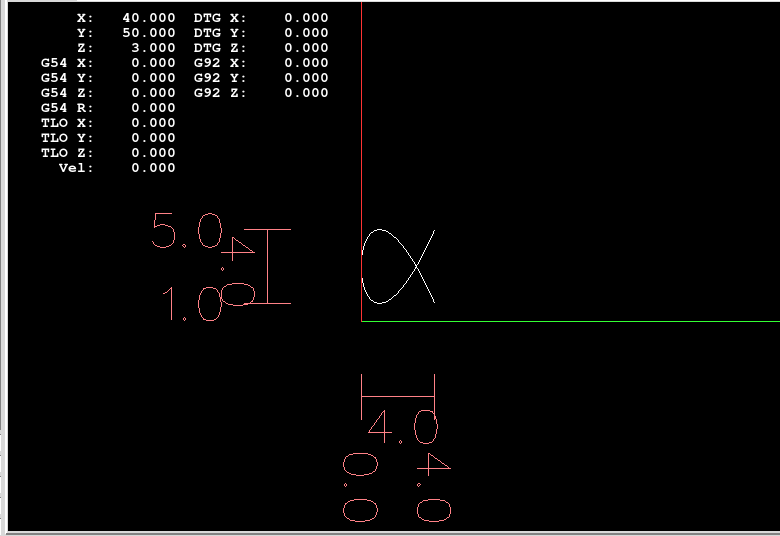
\includegraphics[width=0.560\textwidth]{./07-images/img-Ch5/RIBBON-10L-Axis.png}}
			\frame{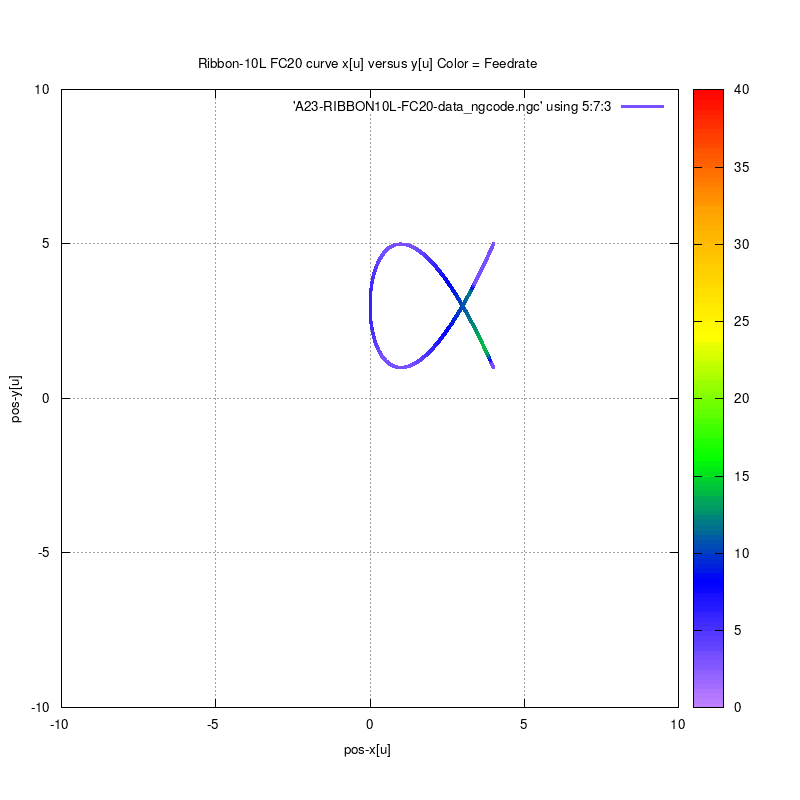
\includegraphics[width=0.394\textwidth]{./07-images/img-Ch5/RIBBON-10L-Feedrate.png}}\\
			
			\rowcolor{LIGHTCYAN}
			\hline \textbf{No. 10 - Ribbon-100L parametric curve}\\
			
			\begin{eqnarray}
		        t(u) & = & 4(u - 0.50) \nonumber \\
	            x(u) & = & 10t^2 \nonumber \\   
	            y(u) & = & 10t^3 - 30t + 30 \nonumber \\
	            u & \in & [0.0, 1.0] \nonumber
			\end{eqnarray}
			
			
			Open ended curve (10 times larger than RIBBON-10L)\\
			Overall Single loop, smooth convex curves\\
			Reflection x-axis: non-symmetrical\\
			Reflection y-axis: non-symmetrical\\
			\frame{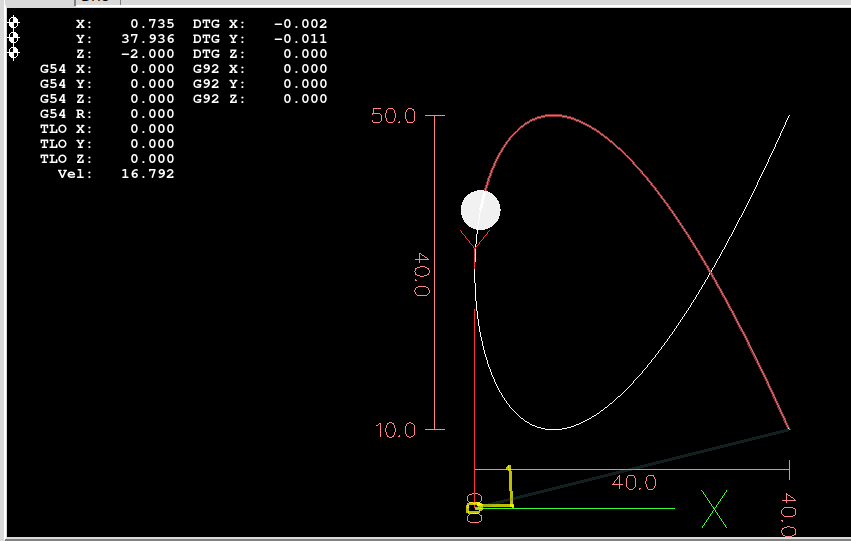
\includegraphics[width=0.575\textwidth]{./07-images/img-Ch5/RIBBON-100L-Axis.png}}
			\frame{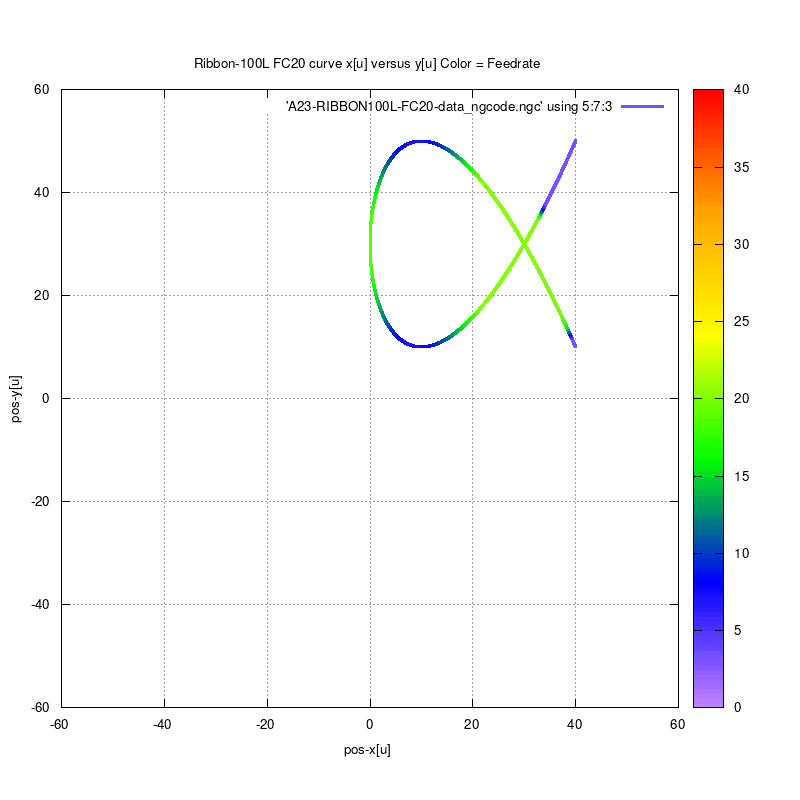
\includegraphics[width=0.370\textwidth]{./07-images/img-Ch5/RIBBON-100L-Feedrate.png}}\\
			
			\hline
		\end{tabular}
		%% \caption{Equations and dimensions of Teardrop and Butterfly curves}		
		\label{table:Part5of5 Equations and dimensions of the parametric curves}
	\end{center}
\end{table}  

\pagebreak

%% ===================================================================
%% \section{Feedrate Plot Profiles}




\pagebreak

%% ===================================================================
%% \section{Algorithm Run Data Summaries} 


%% ===================================================================
\pagebreak
%% \subsection{Teardrop and Butterfly}

\begin{figure}[htbp]
\begin{center}
	\frame{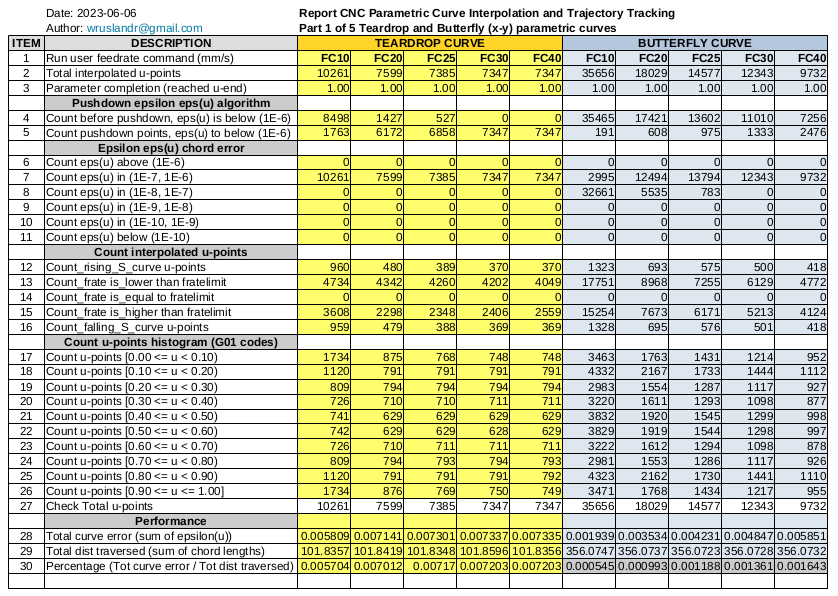
\includegraphics[width=1.00\textwidth]{./07-images/img-Ch52/Teardrop-and-Butterfly-run-data-summary.png}}\\
	\frame{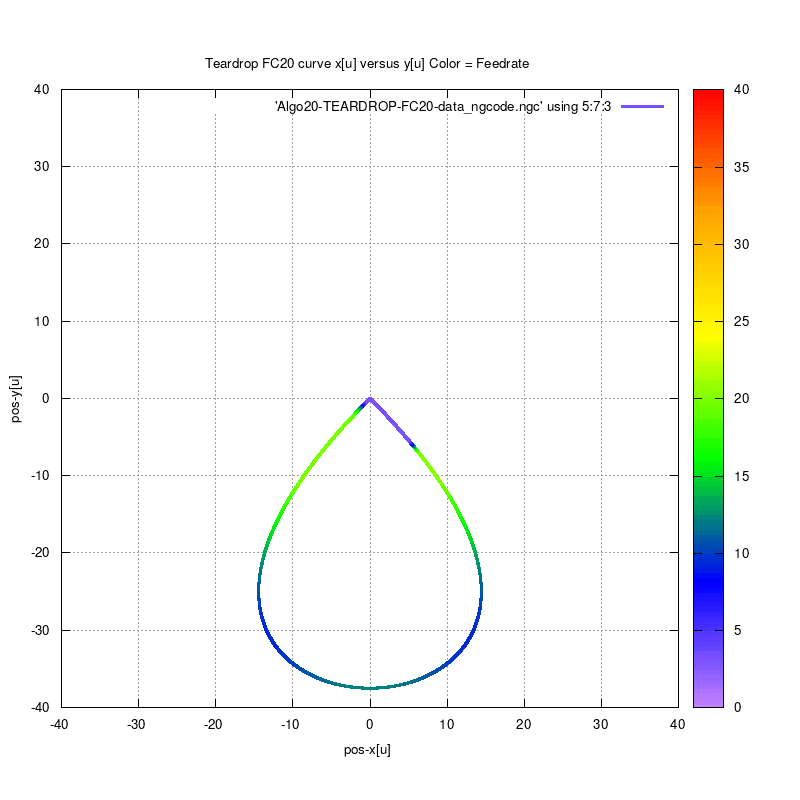
\includegraphics[width=0.49\textwidth]{./07-images/img-Ch5/TEARDROP-Feedrate.png}}
	\frame{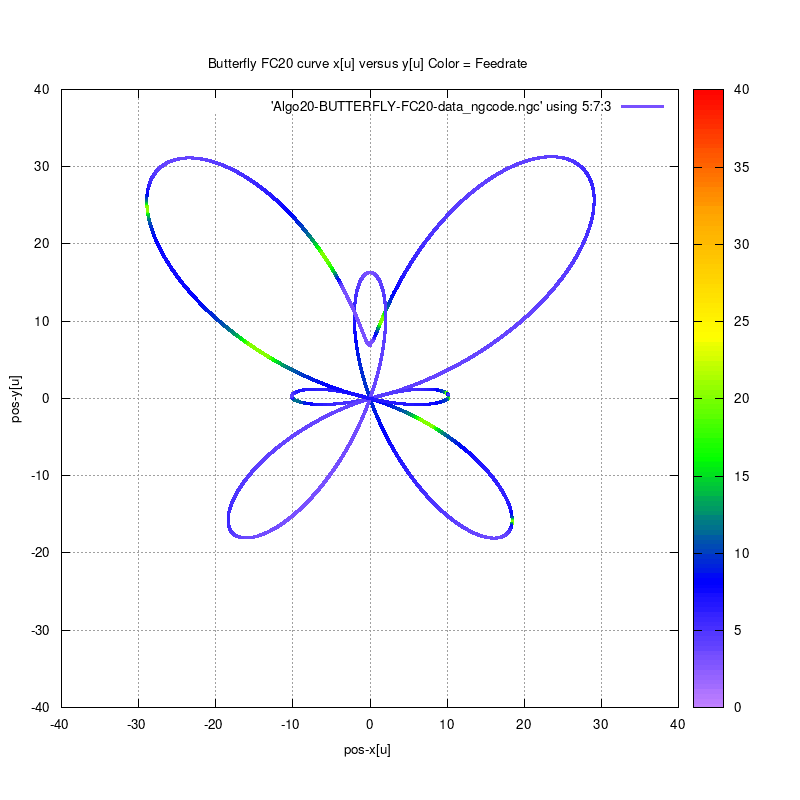
\includegraphics[width=0.49\textwidth]{./07-images/img-Ch5/BUTTERFLY-Feedrate.png}}\\
	\caption{Teardrop and Butterfly run data summary}
	\label{fig:Teardrop and Butterfly run data summary.png}
\end{center}
\end{figure}


%% ===================================================================
\pagebreak
%% \subsection{Ellipse and Skewed-Astroid}
\begin{figure}[htbp]
	\begin{center}
		\frame{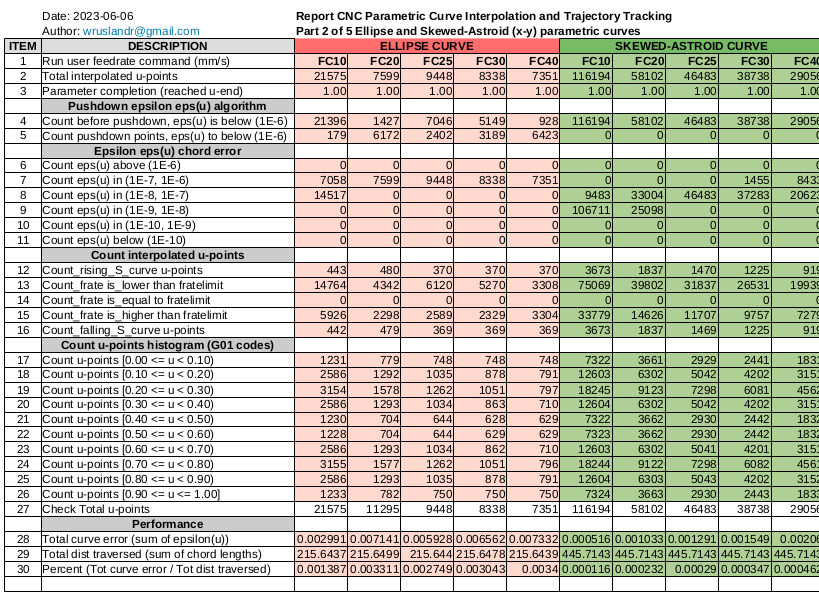
\includegraphics[width=1.00\textwidth]{./07-images/img-Ch52/Ellipse-and-Skewed-Astroid-run-data-summary.png}}\\
		\frame{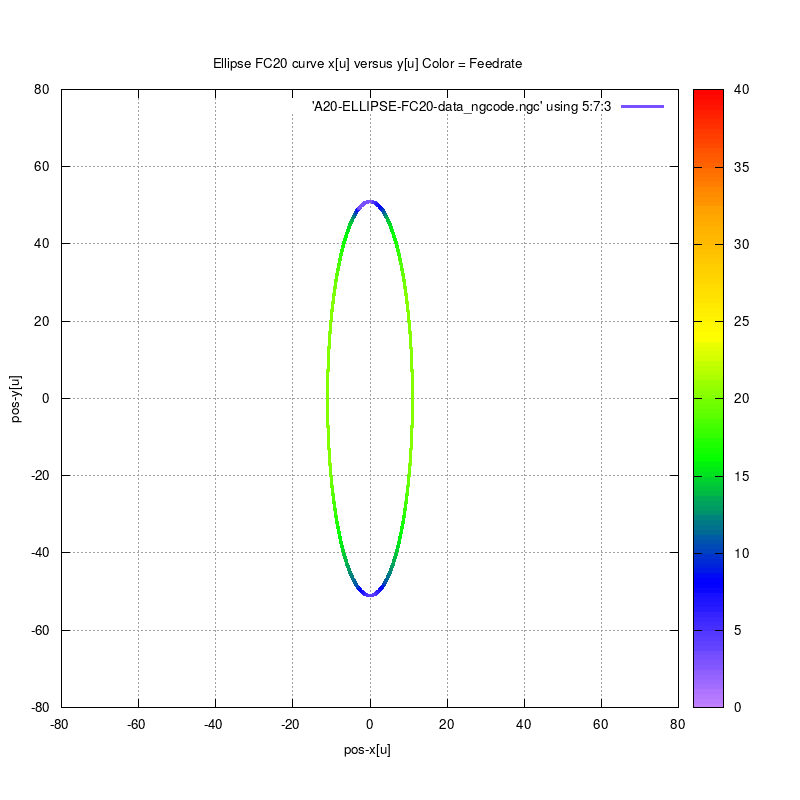
\includegraphics[width=0.49\textwidth]{./07-images/img-Ch5/ELLIPSE-Feedrate.png}}
		\frame{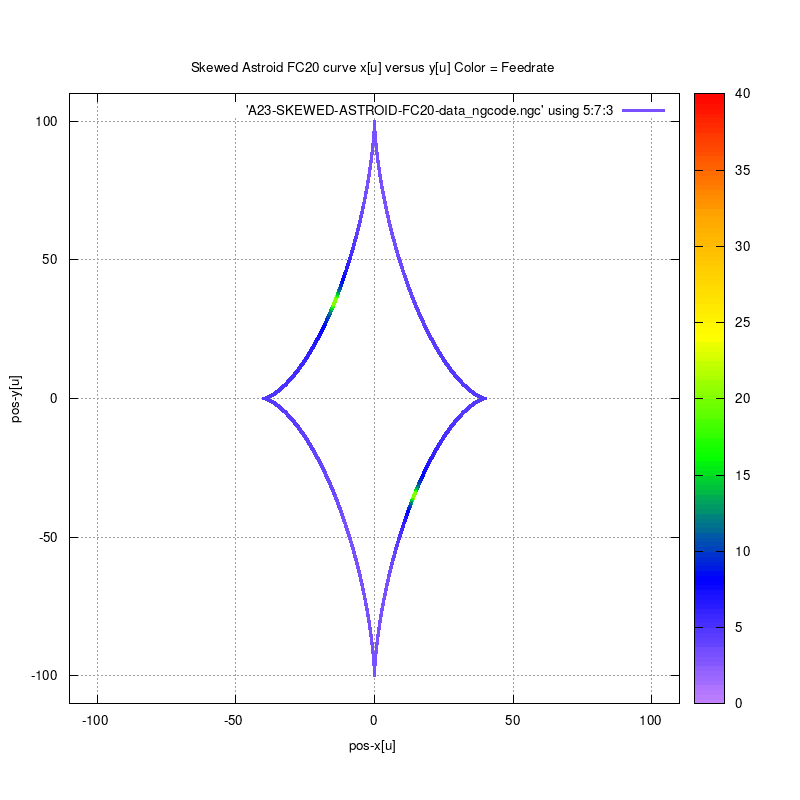
\includegraphics[width=0.49\textwidth]{./07-images/img-Ch5/SKEWED-ASTROID-Feedrate.png}}\\

		\caption{Ellipse and Skewed-Astroid run data summary}
		\label{fig:Ellipse and Skewed-Astroid run data summary.png}
	\end{center}
\end{figure}

%% ===================================================================
\pagebreak
%% \subsection{Circle and AstEpi}
\begin{figure}[htbp]
	\begin{center}
		\frame{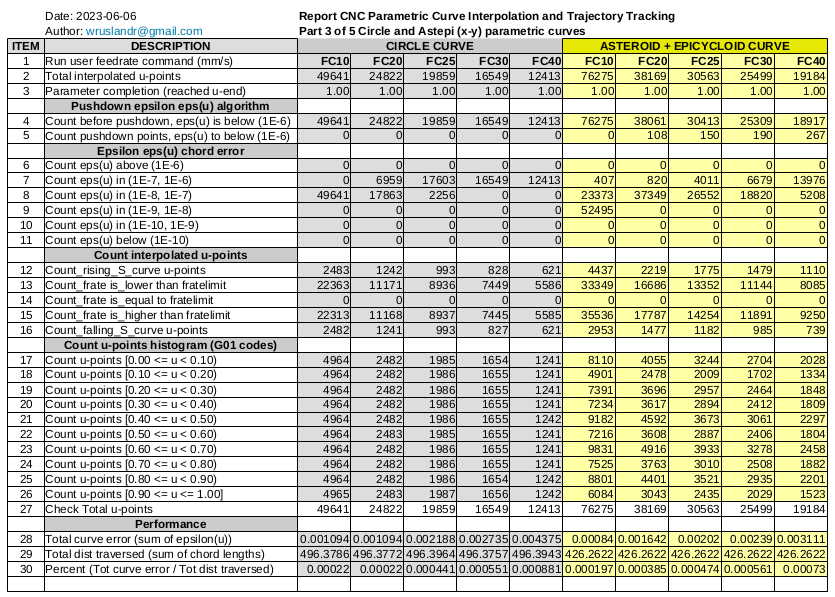
\includegraphics[width=1.00\textwidth]{./07-images/img-Ch52/Circle-and-AstEpi-run-data-summary.png}}\\
		\frame{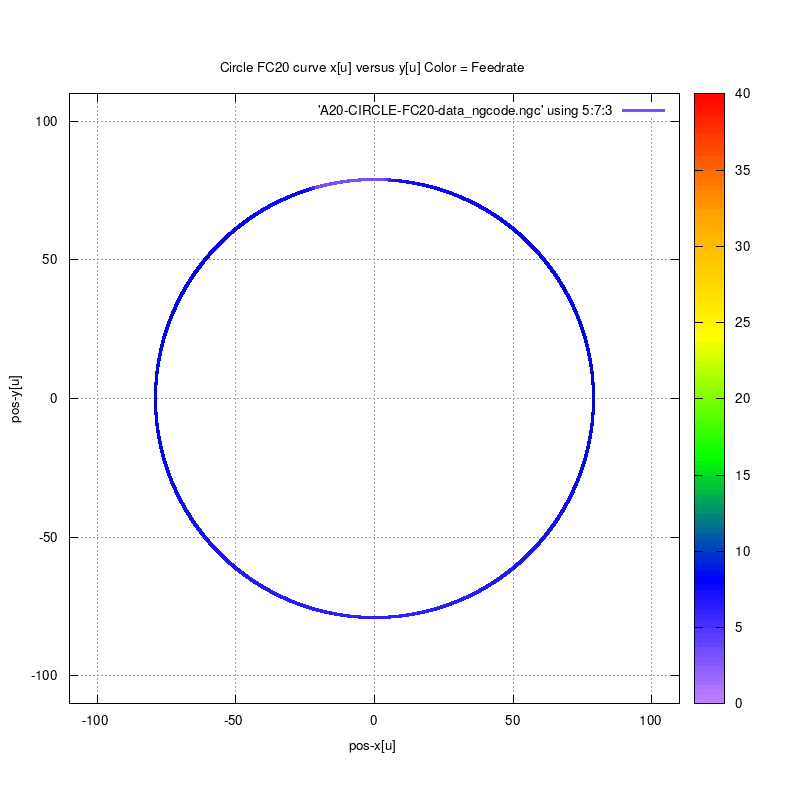
\includegraphics[width=0.49\textwidth]{./07-images/img-Ch5/CIRCLE-Feedrate.png}}
        \frame{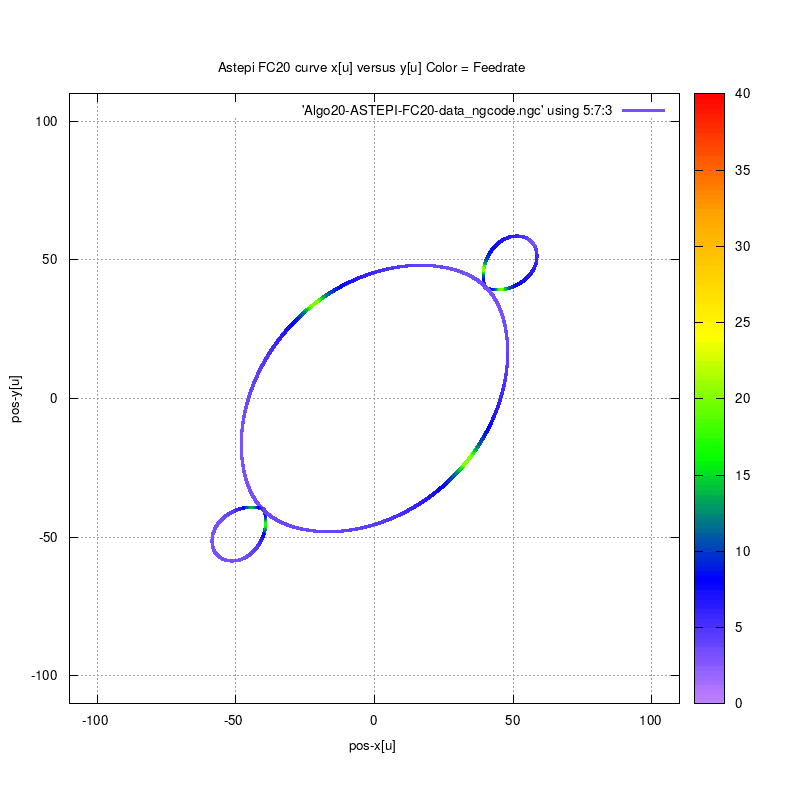
\includegraphics[width=0.49\textwidth]{./07-images/img-Ch5/ASTEPI-Feedrate.png}}\\
		
		\caption{Circle and AstEpi run data summary}
		\label{fig:Circle and AstEpi run data summary.png}
	\end{center}
\end{figure}

\pagebreak
%% \subsection{Snailshell and SnaHyp}
\begin{figure}[htbp]
	\begin{center}
		\frame{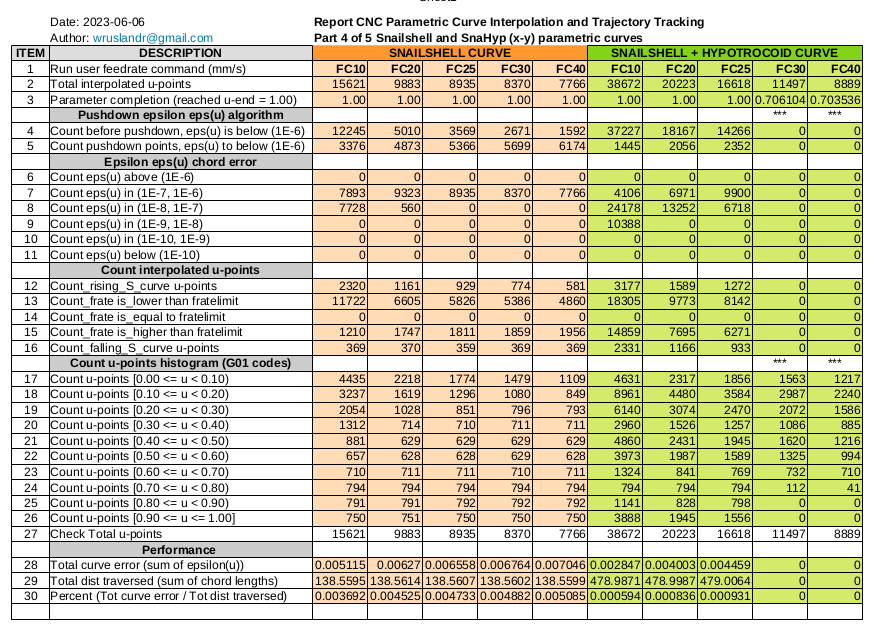
\includegraphics[width=1.00\textwidth]{./07-images/img-Ch52/Snailshell-and-SnaHyp-run-data-summary.png}}\\
		\frame{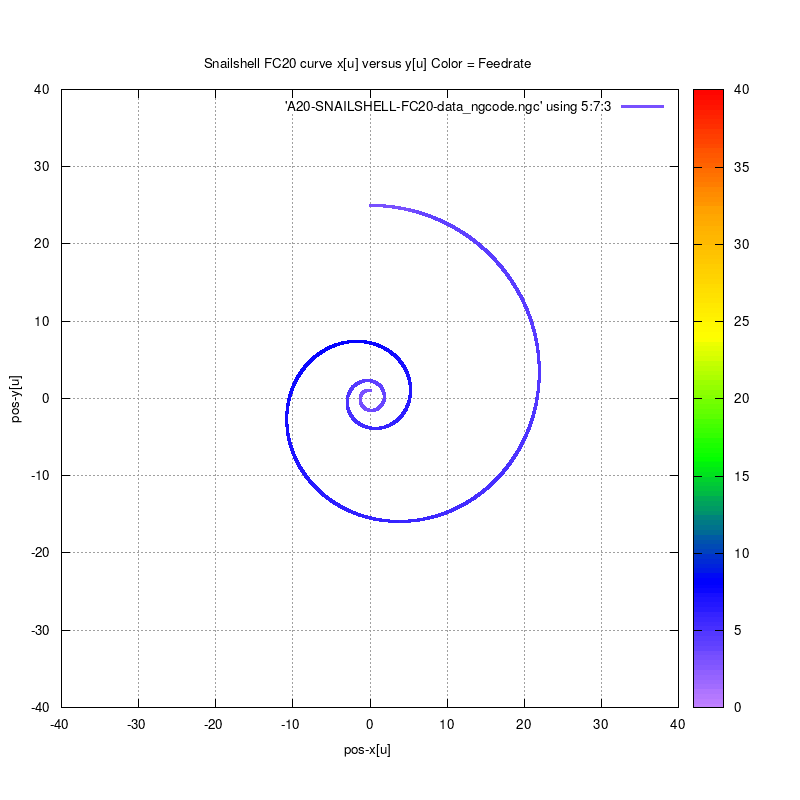
\includegraphics[width=0.49\textwidth]{./07-images/img-Ch5/SNAILSHELL-Feedrate.png}}
        \frame{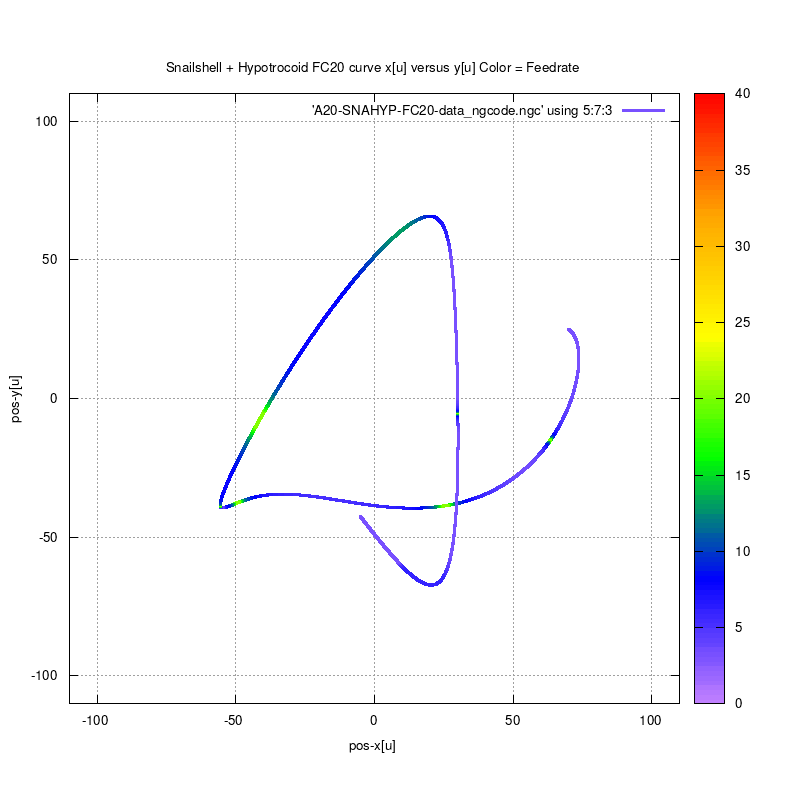
\includegraphics[width=0.49\textwidth]{./07-images/img-Ch5/SNAHYP-Feedrate.png}}\\

		\caption{Snailshell and SnaHyp run data summary}
		\label{fig:Snailshell and SnaHyp run data summary.png}
	\end{center}
\end{figure}



%% ===================================================================
\pagebreak
%% \subsection{Ribbon-10L and Ribbon-100L}
\begin{figure}[htbp]
	\begin{center}
		\frame{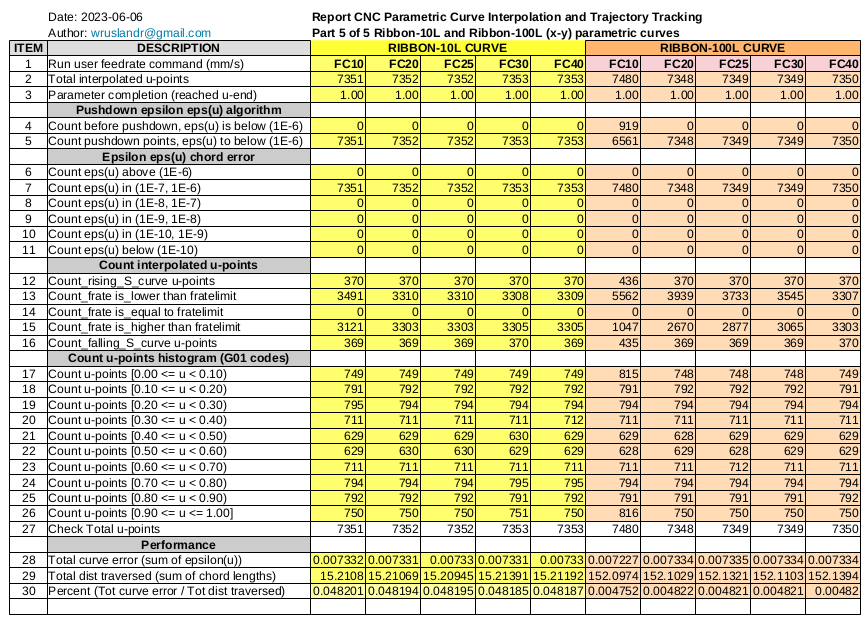
\includegraphics[width=1.00\textwidth]{./07-images/img-Ch52/Ribbon-10L-and-Ribbon-100L-run-data-summary.png}}\\
		\frame{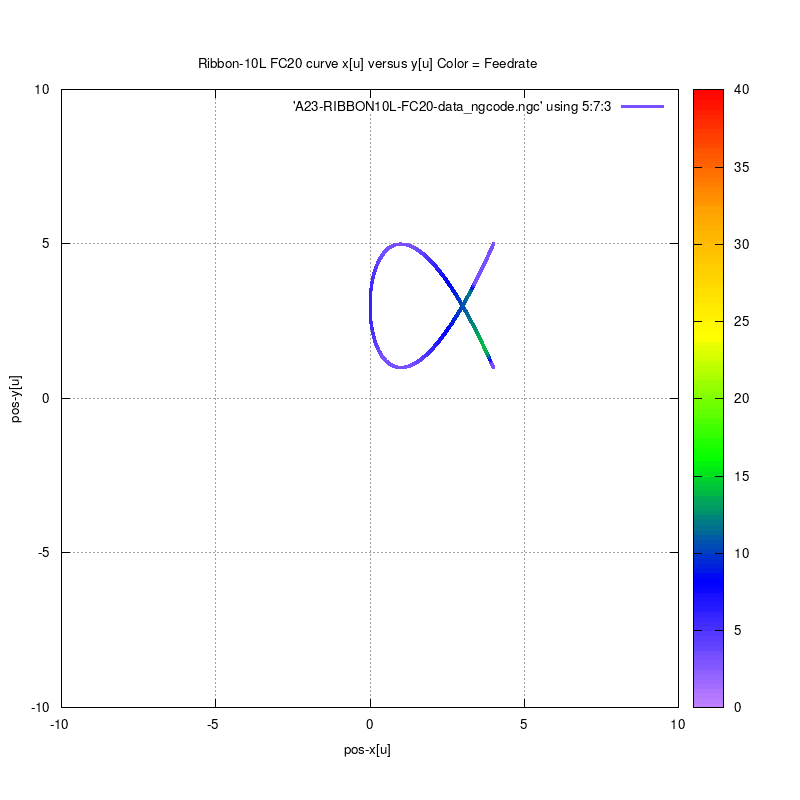
\includegraphics[width=0.49\textwidth]{./07-images/img-Ch5/RIBBON-10L-Feedrate.png}}
        \frame{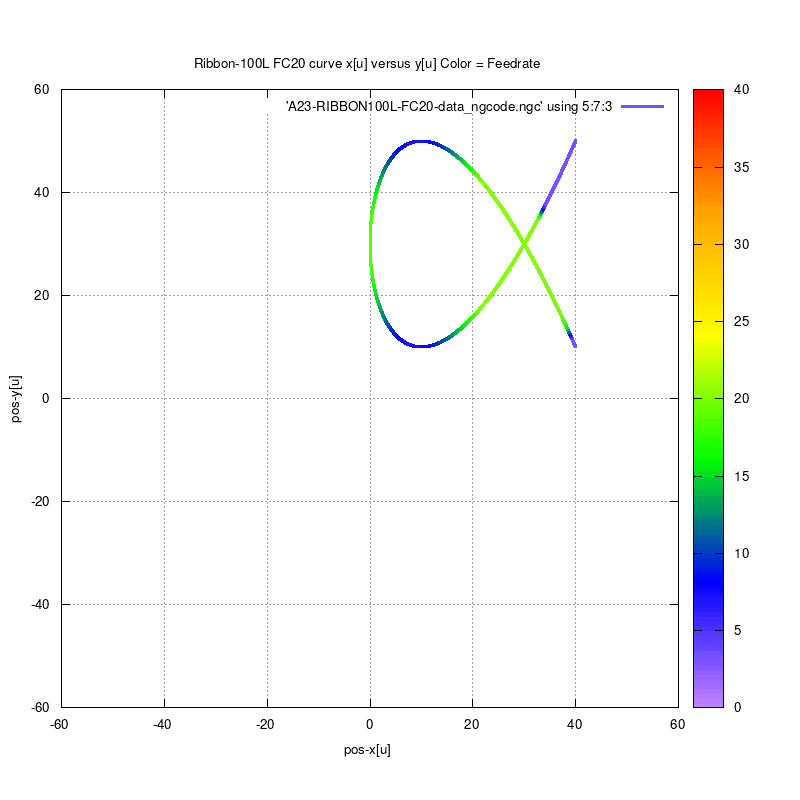
\includegraphics[width=0.49\textwidth]{./07-images/img-Ch5/RIBBON-100L-Feedrate.png}}\\

		\caption{Ribbon-10L and Ribbon-100L run data summary}
		\label{fig:Ribbon-10L and Ribbon-100L run data summary.png}
	\end{center}
\end{figure}


\pagebreak
%% =============================================================

%% \section{Run Feedrate Profiles}











%%
%% \begin{figure}[htbp]
%% \begin{center}
%%	\frame{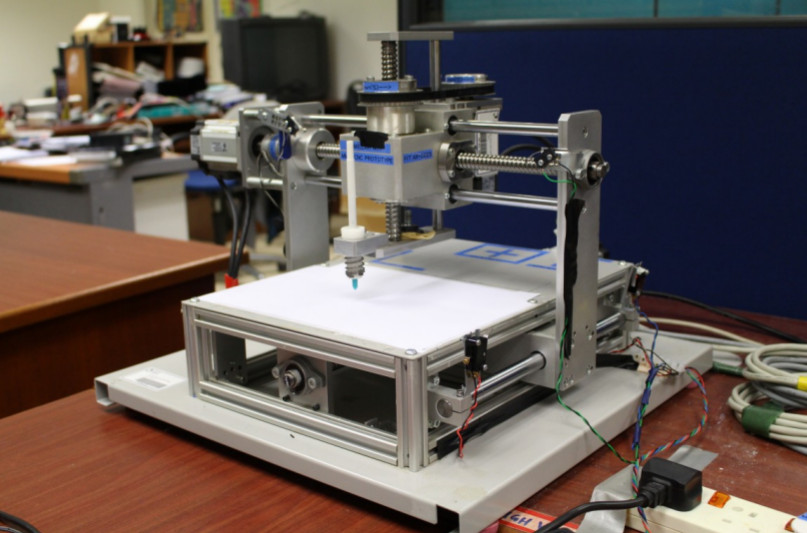
\includegraphics[width=0.85\textwidth]{./07-images/img-Ch4/CNC-Research-Machine-3-Axis.jpg}}
%%	\caption{The UMP 3-axis CNC Research Machine}
%%	\label{fig:CNC-Research-Machine-3-Axis.jpg}
%% \end{center}
%% \end{figure}



% ================== END CHAPTER-5 ========================